\documentclass[
  lualatex, ja=standard, paper={182mm,257mm}, twocolumn, fontsize=8.5pt, baselineskip=13.5pt,
  line_length=24zw, column_gap=6.1mm, number_of_lines=45, head_space=24.5mm, gutter=16.25mm
]{jlreq}
\usepackage[haranoaji]{luatexja-preset}
\usepackage{luatexja-fontspec}
\setmainfont{TeX Gyre Termes}
\setsansfont{TeX Gyre Heros}
\usepackage{graphicx}
\usepackage{booktabs}
\usepackage{array}
\usepackage{xurl}
\urlstyle{same}
\usepackage[hidelinks]{hyperref}
\usepackage{fancyhdr}
\usepackage{microtype}
\usepackage{needspace}
\setlength{\parindent}{1\zw}
\setlength{\columnsep}{6.1mm}
\newcommand{\tablefont}{\fontsize{7.5pt}{10.5pt}\selectfont}
\renewcommand{\floatpagefraction}{0.7}
\renewcommand{\topfraction}{0.9}
\pagestyle{fancy}
\fancyhf{}
\renewcommand{\headrulewidth}{0pt}
\fancyfoot[L]{\fontsize{7.5pt}{9pt}\selectfont 教育情報分析研究会\hspace{1em}生成AI論文\hspace{1em}2026}
\fancyfoot[R]{\fontsize{9pt}{11pt}\selectfont\thepage}
\fancypagestyle{plain}{\fancyhf{}\renewcommand{\headrulewidth}{0pt}%
  \fancyfoot[L]{\fontsize{7.5pt}{9pt}\selectfont 教育情報分析研究会\hspace{1em}生成AI論文\hspace{1em}2026}\fancyfoot[R]{\fontsize{9pt}{11pt}\selectfont\thepage}}
\newcommand{\chap}[2]{\par\vspace{13.5pt}\needspace{4\baselineskip}{\centering\gtfamily\bfseries #1．#2\par}\nopagebreak}
\newcommand{\secn}[3]{\par\needspace{3\baselineskip}{\noindent\gtfamily\bfseries #1.#2.\hspace{1\zw}#3\par}\nopagebreak}
\newcommand{\chapspaced}[1]{\par\vspace{13.5pt}\needspace{4\baselineskip}{\centering\gtfamily\bfseries #1\par}\nopagebreak}

\begin{document}
\twocolumn[{%
\noindent\fbox{\parbox[c][16pt][c]{62mm}{\centering\gtfamily\fontsize{9pt}{16pt}\selectfont 生成AI論文}}\hfill{\fontsize{8pt}{12pt}\selectfont 教育情報分析研究会\hspace{1em}生成AI論文\hspace{1em}2026}\par
\vspace{14pt}{\centering\gtfamily\bfseries\fontsize{13pt}{20pt}\selectfont アンプラグド活動はプログラミング的思考を育てるか：メタ分析\textsuperscript{†}\par}\vspace{10pt}
{\raggedleft\gtfamily\bfseries\fontsize{10pt}{15pt}\selectfont 教育情報分析研究会\hspace{4mm}\par}\vspace{10pt}
\begin{center}\parbox{\dimexpr\textwidth-12mm\relax}{\setlength{\parindent}{1\zw}早期教育におけるプログラミング的思考スキルの育成は重要性を増しており，学校は多様な指導法を模索している．国内外のオープンアクセス論文から条件に合う６本 (参加者450人) を自動で選別・抽出し，数値を本文と照合したうえでランダム効果モデルにより統合した．統合値は \textit{g} = 0.51，95\%信頼区間 [\ensuremath{-}0.15, 1.16]，\textit{I}² = 80.9\% であった．アンプラグド活動はプログラミング的思考の育成に一定の可能性を示すが，小中学校での効果検証にはさらなる厳密な研究が必要である．\par
{\gtfamily キーワード}：メタ分析，アンプラグド活動，プログラミング的思考，初等教育，コンピュータサイエンス教育\par}\end{center}\vspace{4pt}
}]
{\makeatletter\renewcommand{\thefootnote}{}\let\@makefnmark\@empty\footnotetext{\fontsize{7.5pt}{11pt}\selectfont 2026年10月4日公開}\makeatother}
\renewcommand{\thefootnote}{†}\footnotetext{\fontsize{7.5pt}{11pt}\selectfont Society for Educational Data Analysis (SEDA)：Effects of Unplugged Activities on Computational Thinking in School Students: A Meta-Analysis}
\chap{1}{はじめに}
小学校や中学校では，デジタル社会に向けて児童生徒を準備させるために，コンピュータサイエンスの概念をカリキュラムに組み込む動きが強まっている．早期におけるプログラミング的思考 (computational thinking) の育成は，問題解決能力や論理的思考力を養うために不可欠であると考えられている．しかし，学校はコンピュータやインターネット環境の不足といった資源の制約に直面することが多く，これがデジタル機器を用いたプログラミング授業の実施を妨げる要因となっている．

これらの課題に対処するため，教育者はアンプラグド (コンピュータを使わない) コンピュータサイエンスおよびプログラミング的思考活動に注目してきた．これらの活動では，デジタルデバイスを必要とせず，身体的なゲーム，パズル，カード，または身体運動を用いて，アルゴリズム，パターン，デバッグなどの核心的な概念を指導する．研究者は，一般的なプログラミング的思考活動 (BRACKMANN \textit{et al.} 2019，MONTES-LEÓN \textit{et al.} 2020)，コーディング課題 (NAMLI and AYBEK 2022)，Tospaaなどの特定のツール (YILMAZ and İZMIRLI 2023)，Bebrasチャレンジに基づく音楽活動 (DURÁN \textit{et al.} 2023)，SmartGamesなどの教育用ボードゲーム (FANCHAMPS \textit{et al.} 2023) を含む，さまざまなアンプラグドのアプローチを調査してきた．

個々の研究は肯定的またはまちまちな結果を報告しているが，その知見は小規模なサンプルサイズや多様な対照群によって制限されていることが多い．対照群は，通常の授業 (MONTES-LEÓN \textit{et al.} 2020，NAMLI and AYBEK 2022) やプログラミング的思考の指導なし (BRACKMANN \textit{et al.} 2019，DURÁN \textit{et al.} 2023) から，プラグド (コンピュータを用いる) プログラミング (FANCHAMPS \textit{et al.} 2023，YILMAZ and İZMIRLI 2023) まで多岐にわたる．これらの異なる知見を体系的に統合し，全体的な効果量 (effect size) を推定し，異なる教育文脈におけるアンプラグド活動の一貫性を評価するためには，量的な統合が有用である．

本メタ分析の目的は，アンプラグド活動の効果に関する既存の実証的証拠を統合することである．具体的には，本研究は次のリサーチクエスチョンに対処する：対照群と比較して，アンプラグドのコンピュータサイエンスおよびプログラミング的思考活動は，児童生徒のプログラミング的思考テストの成績にどのような全体的効果をもたらすか？

\chap{2}{方法}
\secn{2}{1}{文献の検索}
2026年10月４日に，公開されている２つの書誌データベースを検索した．OpenAlex では題名と要旨を対象に次の検索式を用いた：「(unplugged) AND (“computational thinking” OR programming OR “computer science”) AND (elementary OR primary OR “middle school” OR “junior high” OR secondary OR “K-12” OR grade OR children OR pupils)」．対象は2012年以降に刊行されたオープンアクセスの学術誌論文で，分野が教育学 (Education) または発達・教育心理学 (Developmental and Educational Psychology) に分類されたものに限った．国内の研究を含めるため，J-STAGE でも要旨を対象に「アンプラグド プログラミング」，「アンプラグド 小学校」のキーワードで検索した (2012年以降)．

\secn{2}{2}{適格基準}
次の条件をすべて満たす研究を対象とした：(a) 対象者：初等・中等学校 (K-12) の児童生徒．小学校および中学校の標本が望ましいが，高等学校の標本も許容する．大学，成人，教員・教員志望者の標本は除く；(b) 扱う要因：アンプラグド (コンピュータを使わない) コンピュータサイエンスまたはプログラミング的思考活動．；(c) 比較の対象：プログラミング的思考の指導なし，通常の授業，またはプラグド (コンピュータを用いる) 活動．；(d) 成果指標：プログラミング的思考テストまたはプログラミング概念テスト．；(e) 標準化平均差を計算できる統計量を報告していること．レビュー，質的研究，一事例実験，比較群のない前後比較のみの研究は除外した．

\secn{2}{3}{選別とデータの抽出}
選別とデータの抽出は自動で行った．大規模言語モデル (gemini-3.6-flash, gemini-3.8-flash, gemini-3.5-flash, gemini-3.5-flash-lite) が，各論文の題名と要旨を適格基準に照らして評価した．評価の高い論文から本文 (PDF) を取得してテキストに変換し，同じモデルが研究の特徴と要約統計量を抽出した．抽出したすべての数値は，本文にその数字が実際に書かれているかをプログラムで照合し，１つでも見つからない研究は統合から除外した．選別と抽出を人が確認する工程はない．条件を満たす研究が10本を超えた場合は，評価の高い10本を用いた．

\secn{2}{4}{効果量}
標準化平均差として Hedges の g を求めた (HEDGES 1981)．事後テストの平均・標準偏差・人数から計算し，それらが報告されていない場合は独立な２群の t 値，分子の自由度が１の F 値，報告された d または g の順に用いた．正の値は介入群の得点が高いことを表す．１研究につき１つの効果量を用いた．

\secn{2}{5}{統計解析}
効果量はランダム効果モデルで統合し，研究間分散 (\textit{τ}²) は DerSimonian–Laird 法で推定した (DERSIMONIAN and LAIRD 1986)．統合値の信頼区間と検定には，研究数が少ない場合に推奨される Hartung–Knapp–Sidik–Jonkman 法 (HKSJ 法) を用いた (HARTUNG and KNAPP 2001，INTHOUT \textit{et al.} 2014)．異質性は Q，\textit{I}² (HIGGINS and THOMPSON 2002)，\textit{τ}²，95\% 予測区間で評価した．学校段階 (小学校：１〜６年，中学校：７〜９年) ごとに２研究以上ある場合は下位集団分析を行った．頑健性は１研究ずつ除いた分析で確かめ，Egger の回帰検定 (EGGER \textit{et al.} 1997) は研究数が10以上の場合にのみ行うこととした．効果の大きさは慣例的な目安で解釈した (COHEN 1988)．計算は標準的な式 (BORENSTEIN \textit{et al.} 2009) に従い，公開した JavaScript のプログラム (\url{https://github.com/k518-2026/MetaAnalysisToWP}) で行った．

\chap{3}{結果}
\secn{3}{1}{研究の選定}
検索の結果，OpenAlex から189件 (検索式に合う189件のうち上位)，J-STAGE から18件を得た．重複を除くと204件であった．要旨のある194件を選別し，21件を適格の可能性ありと判定した．本文を調べた21件のうち，取得または読み取りができなかったものが６件，適格基準を満たさなかったものが５件，統計量が不足していたものが３件，抽出した数値を本文で確認できなかったものが１件，効果量が現実的でない値になったものが０件であった．最終的に６本の研究をメタ分析に含めた．

\secn{3}{2}{研究の特徴}
対象とした研究 (BRACKMANN \textit{et al.} 2019，DURÁN \textit{et al.} 2023，FANCHAMPS \textit{et al.} 2023，MONTES-LEÓN \textit{et al.} 2020，NAMLI and AYBEK 2022，YILMAZ and İZMIRLI 2023) の国，学年，研究デザイン，人数，効果量を表１に示す．参加者は合計450人で，実施国はエクアドル，トルコ，スペイン，オランダ，ブラジルであった．学校段階別では，その他が１本，小学校 (１〜６年) が４本，中学校 (７〜９年) が１本であった．１研究あたりの人数は22〜220人，研究ごとの効果量は \textit{g} = \ensuremath{-}0.64 から \textit{g} = 1.33 まで分布していた．

\begin{table*}[tb]
\centering
{\tablefont \gtfamily 表１\hspace{1em}対象とした研究の概要\par}\vspace{2pt}
{\tablefont\renewcommand{\arraystretch}{1.12}
\begin{tabular}{>{\raggedright\arraybackslash}p{0.2600\dimexpr\textwidth-12\tabcolsep\relax}>{\raggedright\arraybackslash}p{0.1100\dimexpr\textwidth-12\tabcolsep\relax}>{\raggedright\arraybackslash}p{0.1200\dimexpr\textwidth-12\tabcolsep\relax}>{\raggedright\arraybackslash}p{0.2300\dimexpr\textwidth-12\tabcolsep\relax}>{\raggedright\arraybackslash}p{0.0700\dimexpr\textwidth-12\tabcolsep\relax}>{\raggedright\arraybackslash}p{0.2100\dimexpr\textwidth-12\tabcolsep\relax}}
\toprule
研究 & 国 & 学年 & デザイン & \textit{N} & \textit{g} [95\% CI] \\
\midrule
MONTES-LEÓN \textit{et al.} (2020) & エクアドル & 高校1年 & 準実験 & 80 & 0.69 [0.25, 1.14] \\
NAMLI and AYBEK (2022) & トルコ & 小学5年 & 無作為化比較試験 & 54 & 0.37 [\ensuremath{-}0.17, 0.90] \\
YILMAZ and İZMIRLI (2023) & トルコ & 5年生 & 準実験 & 36 & 0.56 [\ensuremath{-}0.09, 1.22] \\
DURÁN \textit{et al.} (2023) & スペイン & 小学3〜6年 & 準実験 & 220 & 1.33 [1.00, 1.67] \\
FANCHAMPS \textit{et al.} (2023) & オランダ & 小学5〜6年 & ランダム化比較試験 & 22 & \ensuremath{-}0.64 [\ensuremath{-}1.47, 0.19] \\
BRACKMANN \textit{et al.} (2019) & ブラジル & 小学5〜6年 & 準実験 & 38 & 0.36 [\ensuremath{-}0.27, 0.98] \\
\bottomrule
\end{tabular}\par}
\vspace{2pt}{\tablefont\noindent 注：CI＝信頼区間．g は Hedges の g（正の値は介入群が高い）．学年・デザインは論文の本文から自動で抽出した．\par}
\end{table*}
各研究の介入，比較の条件，成果指標を表２に示す．６本はいずれも，介入群と比較群を事後テストで比べた研究である．

\begin{table*}[tb]
\centering
{\tablefont \gtfamily 表２\hspace{1em}各研究の介入・比較の条件・成果指標\par}\vspace{2pt}
{\tablefont\renewcommand{\arraystretch}{1.12}
\begin{tabular}{>{\raggedright\arraybackslash}p{0.2000\dimexpr\textwidth-8\tabcolsep\relax}>{\raggedright\arraybackslash}p{0.3200\dimexpr\textwidth-8\tabcolsep\relax}>{\raggedright\arraybackslash}p{0.2400\dimexpr\textwidth-8\tabcolsep\relax}>{\raggedright\arraybackslash}p{0.2400\dimexpr\textwidth-8\tabcolsep\relax}}
\toprule
研究 & 介入 & 比較の条件 & 成果指標 \\
\midrule
MONTES-LEÓN \textit{et al.} (2020) & アンプラグドなプログラミング思考学習活動 & 通常の手理・数学的推論指導 & プログラミング思考テスト \\
NAMLI and AYBEK (2022) & アンプラグド・コーディング活動 & 通常授業（介入なし） & 国際情報科学・計算論的思考タスクテスト（IICTATT） \\
YILMAZ and İZMIRLI (2023) & Tospaaアンプラグドコーディング活動 & Scratchブロックベースコーディング活動 & プログラミング的思考テスト \\
DURÁN \textit{et al.} (2023) & Bebrasチャレンジに基づくアンプラグド音楽活動 & プログラミング的思考の指導なし & Bebras問題を用いたプログラミング的思考テスト \\
FANCHAMPS \textit{et al.} (2023) & アンプラグドのスマートゲーム（SmartGames） & Lego EV-3を使用したプラグインのSRAプログラミング & 計算論的思考テスト（CTt） \\
BRACKMANN \textit{et al.} (2019) & アンプラグドな計算論的思考活動 & 計算論的思考の指導なし & 計算論的思考テスト \\
\bottomrule
\end{tabular}\par}
\vspace{2pt}{\tablefont\noindent 注：論文の本文から自動で抽出し，要約した．\par}
\end{table*}
\secn{3}{3}{全体の効果}
図１に各研究の効果量と統合値をフォレストプロットで示す．四角は各研究の効果量で，大きさは統合における重みを表す．横線は95\%信頼区間，最下段のひし形は統合値である．６本のうち５本で効果量が正の値であり，２本では95\%信頼区間が０を含まなかった．重みが最も大きかったのは DURÁN \textit{et al.} (2023) (19.5\%) であった．

\begin{figure*}[tb]
\centering
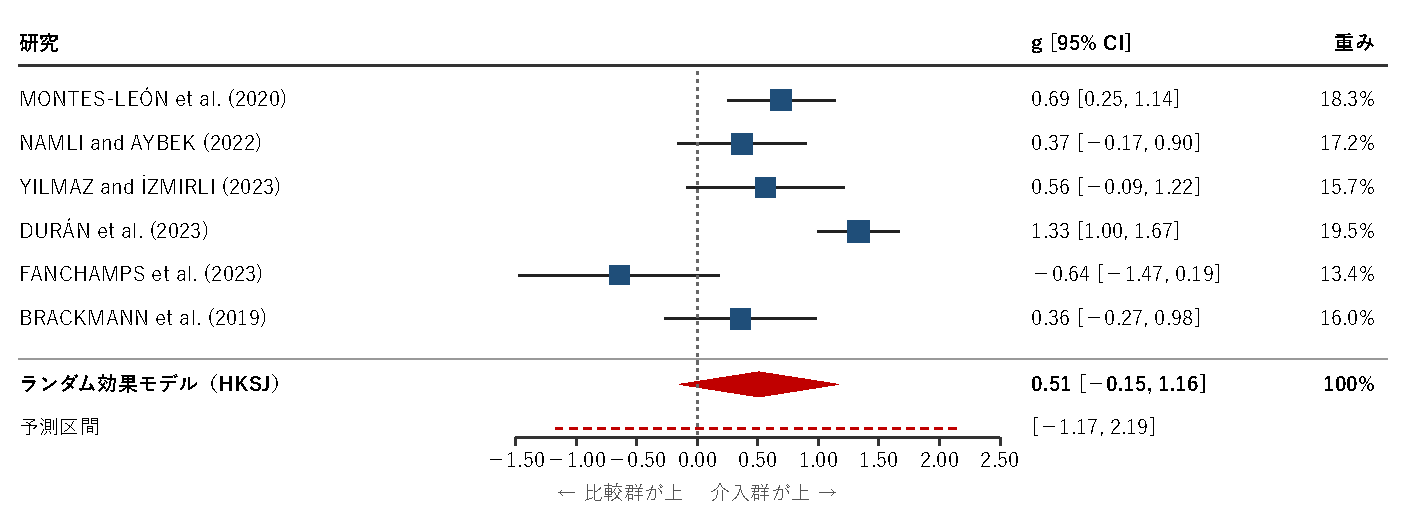
\includegraphics[width=\textwidth]{forest-ja.pdf}\par\vspace{2pt}
{\tablefont\gtfamily 図１\hspace{1em}フォレストプロット\par}{\tablefont 注：四角は各研究の効果量 (大きさは重み)，横線は95\%信頼区間，ひし形は統合値，点線は予測区間を表す．\par}
\end{figure*}
ランダム効果モデルによる統合値は \textit{g} = 0.51，95\% 信頼区間 [\ensuremath{-}0.15, 1.16]，\textit{t}(5) = 2.00，\textit{p} = .103 であった．統計的に有意ではなく (信頼区間が０を含む)，効果がない場合とも矛盾しない．点推定値は慣例的な目安では中程度効果にあたる．固定効果モデルによる推定値は \textit{g} = 0.75 であった．これらの推定値を表３にまとめる．

\secn{3}{4}{異質性}
研究間の異質性は非常に大きかった (\textit{Q}(5) = 26.13，p < .001，\textit{I}² = 80.9\%，\textit{τ}² = 0.302)．95\% 予測区間は \ensuremath{-}1.17 から 2.19 であった．

\secn{3}{5}{下位集団分析と感度分析}
少なくとも一方の学校段階で研究が２本未満だったため，学校段階別の下位集団分析は行わなかった．１研究ずつ除いた推定値は 0.35 から 0.70 の範囲であった．研究数が10未満のため，出版バイアスの検定は行わなかった．

\begin{table*}[tb]
\centering
{\tablefont \gtfamily 表３\hspace{1em}メタ分析の結果\par}\vspace{2pt}
{\tablefont\renewcommand{\arraystretch}{1.12}
\begin{tabular}{lrrrrrrr}
\toprule
モデル & \textit{k} & \textit{N} & \textit{g} & 95\% CI & \textit{p} & \textit{I}² (\%) & \textit{τ}² \\
\midrule
ランダム効果（HKSJ） & 6 & 450 & 0.51 & [\ensuremath{-}0.15, 1.16] & .103 & 80.9 & 0.302 \\
固定効果 & 6 & 450 & 0.75 & [0.55, 0.96] & < .001 & — & — \\
\bottomrule
\end{tabular}\par}
\vspace{2pt}{\tablefont\noindent 注：\textit{k}＝研究数．HKSJ＝Hartung–Knapp–Sidik–Jonkman 法による信頼区間．95\% 予測区間 [\ensuremath{-}1.17, 2.19]．\par}
\end{table*}
\chap{4}{考察}
本メタ分析では，合計サンプルサイズ450名の児童生徒を対象とした６件の研究からデータを統合した．表３に示すように，統合された全体的な効果量は中程度であり，Hedgesのg = 0.51であったが，この効果は統計的に有意ではなかった (95\%信頼区間 [-0.15, 1.16]，\textit{p} = .103)．フォレストプロット (図１) は，\textit{Q}(5) = 26.13，p < .001，I2 = 80.9\%，tau2 = 0.302に示されるように，含まれた研究間に実質的な異質性 (heterogeneity) が存在することを明らかにしている．この高い異質性は，アンプラグド活動の効果が，具体的な実施方法や文脈によって大きく異なることを示唆している．[-1.17, 2.19] という広い予測区間は，今後の実施において，非常に肯定的な結果にも否定的な結果にもなり得ることをさらに強調している．

統合推定値の頑健性を評価するために，１研究除外 (leave-one-out) 感度分析を実施したところ，統合されたHedgesのgは0.35から0.70の範囲となり，特定の単一研究が全体的な効果の方向に不当に大きな影響を与えていないことが示された．学校段階に基づくサブグループ解析は，学校段階あたりの研究数が２件未満であり，信頼性の高い比較が困難であったため実施しなかった．さらに，含まれた研究数が少なかった (10件未満) ため，公表バイアス (publication bias) の評価は行わなかった．

研究の概要を表１に示し，具体的な介入とアウトカムの詳細を表２に示す．個々の研究の効果は大きく異なっていた．例えば，(DURÁN \textit{et al.} 2023) は，指導なしと比較して，Bebrasチャレンジに基づくアンプラグドの音楽活動において非常に大きな正の効果 (\textit{g} = 1.33) を報告した．準実験デザインにおいては，エクアドルの (MONTES-LEÓN \textit{et al.} 2020) (\textit{g} = 0.69) やトルコの (YILMAZ and İZMIRLI 2023) (\textit{g} = 0.56) のように，中程度の正の効果が観察された．対照的に，(FANCHAMPS \textit{et al.} 2023) はアンプラグドのSmartGamesとプラグドのLego EV-３プログラミングを比較した際に負の効果 (\textit{g} = -0.64) を示したが，著者らは同等の発達が見られたと言及している．その他の研究，例えば (NAMLI and AYBEK 2022) (\textit{g} = 0.37) や (BRACKMANN \textit{et al.} 2019) (\textit{g} = 0.36) は，より小さく有意ではない正の傾向を示した．

１〜９年生 (小学校・中学校) の教員にとって，これらの知見は，特にデジタル資源が不足している場合に，アンプラグド活動がプログラミング的思考を指導するための実行可能で低コストな導入部になり得ることを示唆している．しかし，全体的な効果は統計的に有意ではなく，ばらつきが大きいため，教員はアンプラグド活動をプラグドプログラミングの完全な代替物とみなべきではない．むしろ，(DURÁN \textit{et al.} 2023) に見られるようにアンプラグドの授業に身体的または音楽的な要素を取り入れたり，(NAMLI and AYBEK 2022，YILMAZ and İZMIRLI 2023) のようにブロック型プログラミングと組み合わせたりすることが，最もバランスの取れた教育的成果をもたらす可能性がある．

\chap{5}{まとめ}
結論として，本メタ分析は，アンプラグドのコンピュータサイエンス活動が，児童生徒のプログラミング的思考スキルに対して中程度ではあるが統計的に有意ではない全体的効果 (\textit{g} = 0.51) を持つことを示している．高い異質性と広い予測区間は，実践におけるこれらの介入の多様な成果を強調している．アンプラグド活動は，小中学校の教員にとって有望で取り組みやすいツールを提供するが，その効果を最大化する具体的な条件や設計を特定するためには，さらなる厳密かつ大規模な研究が不可欠である．

いくつかの限界を考慮する必要がある．第一に，本メタ分析は非常に少ない研究数 (６件，\textit{N} = 450) に基づいているため，有意な全体的効果を検出するための統計的検出力が制限され，頑健なサブグループ解析や公表バイアス解析の実施が困難であった．第二に，データが自動的に抽出されたため，軽微な不正確さが生じたり，文脈の微妙な詳細が見落とされたりした可能性がある．

さらに，含まれた研究は，ランダム化比較試験 (FANCHAMPS \textit{et al.} 2023，NAMLI and AYBEK 2022) から準実験デザイン (BRACKMANN \textit{et al.} 2019，DURÁN \textit{et al.} 2023，MONTES-LEÓN \textit{et al.} 2020，YILMAZ and İZMIRLI 2023) に至るまで，多様な研究デザインを採用していた．アウトカムの測定尺度も異なっており，Bebrasタスク (DURÁN \textit{et al.} 2023) や一般的なプログラミング的思考テスト (BRACKMANN \textit{et al.} 2019，FANCHAMPS \textit{et al.} 2023，MONTES-LEÓN \textit{et al.} 2020，YILMAZ and İZMIRLI 2023) など，異なるプログラミング的思考テストが使用されており，これらは同じ潜在的構成概念を捉えていない可能性がある．最後に，標本は主に小学校の学年 (BRACKMANN \textit{et al.} 2019，DURÁN \textit{et al.} 2023，FANCHAMPS \textit{et al.} 2023，NAMLI and AYBEK 2022，YILMAZ and İZMIRLI 2023) に集中しており，10年生 (高校１年生) を対象とした研究は１件のみ (MONTES-LEÓN \textit{et al.} 2020) であったため，K-12 (幼稚園から高校まで) のすべての学校段階における知見の一般化可能性は制限される．

加えて，本分析は選別とデータ抽出を言語モデルで自動化しており，抽出した数値は本文との文字列の照合でしか確認していない．数値が本文に存在しても，別の群や別の測定の値を取り違えている可能性は残る．対象はオープンアクセスで本文を取得できた論文に限られ，有料の論文や未刊行の研究は含まれていない．

\chapspaced{付\hspace{1\zw}記}
本論文は，教育情報分析研究会が生成AIを用いて自動で作成した「生成AI論文」である．文献の選別，データの抽出，はじめに・考察・まとめの文章の作成には大規模言語モデル (gemini-3.6-flash, gemini-3.8-flash, gemini-3.5-flash, gemini-3.5-flash-lite) を用い，統計量はすべてプログラムで計算した．査読は受けていない．

同じ内容の英語版がある (\url{https://raw.githubusercontent.com/k518-2026/MetaAnalysisToWP/main/reports/2026-10-04-info-unplugged-ct/paper-en.pdf})．抽出したデータとプログラムは \url{https://github.com/k518-2026/MetaAnalysisToWP} で公開している．

\chapspaced{参考文献}
{\noindent * はメタ分析に含めた研究を示す．\par}
{\small
\par\noindent\hangindent=2\zw\hangafter=1 BORENSTEIN, M., HEDGES, L. V., HIGGINS, J. P. T. and ROTHSTEIN, H. R. (2009) \textit{Introduction to Meta-Analysis}. Wiley. \url{https://doi.org/10.1002/9780470743386}\par
\par\noindent\hangindent=2\zw\hangafter=1 *BRACKMANN, C. P., BARONE, D. A. C., BOUCINHA, R. M. and REICHERT, J. T. (2019) Development of Computational Thinking in Brazilian Schools with Social and Economic Vulnerability. \textit{International Journal for Innovation Education and Research}, \textbf{7} (4)：79-96. \url{https://doi.org/10.31686/ijier.vol7.iss4.1390}\par
\par\noindent\hangindent=2\zw\hangafter=1 COHEN, J. (1988) \textit{Statistical Power Analysis for the Behavioral Sciences} (2nd ed.). Lawrence Erlbaum Associates\par
\par\noindent\hangindent=2\zw\hangafter=1 DERSIMONIAN, R. and LAIRD, N. (1986) Meta-analysis in clinical trials. \textit{Controlled Clinical Trials}, \textbf{7} (3)：177-188. \url{https://doi.org/10.1016/0197-2456(86)90046-2}\par
\par\noindent\hangindent=2\zw\hangafter=1 *DURÁN, C. M. S., GARCÍA-FERNÁNDEZ, C. M. and GALÁN, A. A. (2023) Alfabetización Computacional: Actividades musicales desenchufadas sobre el Desafío Internacional de Bebras. \textit{Revista de Educación a Distancia (RED)}, \textbf{23} (73). \url{https://doi.org/10.6018/red.540191}\par
\par\noindent\hangindent=2\zw\hangafter=1 EGGER, M., DAVEY SMITH, G., SCHNEIDER, M. and MINDER, C. (1997) Bias in meta-analysis detected by a simple, graphical test. \textit{BMJ}, \textbf{315} (7109)：629-634. \url{https://doi.org/10.1136/bmj.315.7109.629}\par
\par\noindent\hangindent=2\zw\hangafter=1 *FANCHAMPS, N. L. J. A., VAN GOOL, E., SLANGEN, L. and HENNISSEN, P. (2023) The effect on computational thinking and identified learning aspects: Comparing unplugged smartGames with SRA-Programming with tangible or On-screen output. \textit{Education and Information Technologies}, \textbf{29} (3)：2999-3024. \url{https://doi.org/10.1007/s10639-023-11956-6}\par
\par\noindent\hangindent=2\zw\hangafter=1 HARTUNG, J. and KNAPP, G. (2001) A refined method for the meta-analysis of controlled clinical trials with binary outcome. \textit{Statistics in Medicine}, \textbf{20} (24)：3875-3889. \url{https://doi.org/10.1002/sim.1009}\par
\par\noindent\hangindent=2\zw\hangafter=1 HEDGES, L. V. (1981) Distribution theory for Glass's estimator of effect size and related estimators. \textit{Journal of Educational Statistics}, \textbf{6} (2)：107-128. \url{https://doi.org/10.3102/10769986006002107}\par
\par\noindent\hangindent=2\zw\hangafter=1 HIGGINS, J. P. T. and THOMPSON, S. G. (2002) Quantifying heterogeneity in a meta-analysis. \textit{Statistics in Medicine}, \textbf{21} (11)：1539-1558. \url{https://doi.org/10.1002/sim.1186}\par
\par\noindent\hangindent=2\zw\hangafter=1 INTHOUT, J., IOANNIDIS, J. P. A. and BORM, G. F. (2014) The Hartung-Knapp-Sidik-Jonkman method for random effects meta-analysis is straightforward and considerably outperforms the standard DerSimonian-Laird method. \textit{BMC Medical Research Methodology}, \textbf{14}：25. \url{https://doi.org/10.1186/1471-2288-14-25}\par
\par\noindent\hangindent=2\zw\hangafter=1 *MONTES-LEÓN, H., NEIRA, R. H., PÉREZ-MARÍN, D. and LEÓN, S. R. M. (2020) Improving Computational Thinking in Secondary Students with Unplugged Tasks. \textit{Education in the Knowledge Society (EKS)}, \textbf{21}：12. \url{https://doi.org/10.14201/eks.23002}\par
\par\noindent\hangindent=2\zw\hangafter=1 *NAMLI, N. A. and AYBEK, B. (2022) An Investigation of The Effect of Block-Based Programming and Unplugged Coding Activities on Fifth Graders’ Computational Thinking Skills, Self-Efficacy and Academic Performance. \textit{Contemporary Educational Technology}, \textbf{14} (1)：ep341. \url{https://doi.org/10.30935/cedtech/11477}\par
\par\noindent\hangindent=2\zw\hangafter=1 *YILMAZ, T. and İZMIRLI, S. (2023) Effect of unplugged and plugged coding activities on secondary school students’ computational thinking skills. \textit{Journal of Educational Technology and Online Learning}, \textbf{6} (4)：1180-1193. \url{https://doi.org/10.31681/jetol.1375335}\par
}
\chapspaced{Summary}
{\setlength{\parindent}{1\zw}\noindent Developing computational thinking skills in early education is increasingly vital, prompting schools to explore diverse pedagogical approaches. Using an automated workflow in which every extracted number was verified against the full text, 6 open-access studies (\textit{N} = 450) were pooled with a random-effects model. The pooled effect was \textit{g} = 0.51, 95\% CI [\ensuremath{-}0.15, 1.16], with \textit{I}² = 80.9\%. Unplugged activities show moderate potential for fostering computational thinking, but further rigorous research is required to confirm their effectiveness in primary and lower secondary classrooms.\par
KEYWORDS: META-ANALYSIS, UNPLUGGED ACTIVITIES, COMPUTATIONAL THINKING, ELEMENTARY EDUCATION, COMPUTER SCIENCE EDUCATION\par}
\end{document}
